\documentclass[aspectratio=169, table]{beamer}


%\usepackage[beamertheme=./praditatheme]{Pradita}

\graphicspath{{../../images/}}

\usetheme{Pradita}

\title{Chapter-01:\\Introduction to Software Architecture\\and Client-Server Architecture}
\subtitle{IF231303-Software Architecture}
\author{Alfa Yohannis}
\begin{document}
	
	\begin{frame}[plain]
		\maketitle
	\end{frame}
	
	
	\begin{frame}{Introduction}
		\begin{itemize}
			\item Software architecture defines the structure, components, and relationships within a system.
			\item Plays a crucial role in scalability, reliability, security, and application maintenance.
			\item As system complexity increases, choosing the right architecture is key to success.
			\item Core principles: modularity, scalability, performance, security, and maintainability.
			\item Implementation techniques: layered architecture, microservices, and event-driven.
			\item Case studies: Netflix, Healthcare.gov, and event-driven banking.
			\item Common communication model: Client-Server architecture.
		\end{itemize}
	\end{frame}
	
	\begin{frame}{Case Studies and Architectural Models}
		\begin{itemize}
			\item Netflix architecture transformation: monolithic to microservices.
			\item Impact of poor architecture: Healthcare.gov failure.
			\item Event-driven banking for real-time transaction processing.
			\item Client-Server architecture: background, structure, advantages, and disadvantages.
			\item Client-Server implementation in various business scenarios.
			\item Adapting architectural models based on technical and business needs.
		\end{itemize}
	\end{frame}
	
	\begin{frame}{Topics}
		\begin{columns}
			\column{0.5\textwidth}
			\begin{enumerate}
				\item Introduction to Software Architecture and Client-Server Architecture
				\item Containers
				\item Layered Architecture
				\item Model-View-* (MV*) Architecture
				\item Hexagonal Architecture
				\item Microkernel Architecture
				\item Peer-to-Peer (P2P) Architecture
			\end{enumerate}
			
			\column{0.5\textwidth}
			\begin{enumerate}
				\setcounter{enumi}{7}
				\item Space-Based Architecture (SBA)
				\item Microservices Architecture
				\item Event-Driven Architecture (EDA)
				\item Pipeline / Pipe-and-Filter Architecture
				\item Orchestration-driven Service-Oriented Architecture (ODSOA)
				\item Service-based (Serverless) Architecture
				\item DevOps
			\end{enumerate}
		\end{columns}
	\end{frame}
	
	
	\begin{frame}{Definition of Software Architecture}
		\begin{itemize}
			\item Software architecture is the fundamental structure of a software system.
			\item Comprises software components, their relationships, and design principles.
			\item IEEE Standard 1471-2000 defines software architecture as:
		\end{itemize}
		\begin{quote}
			"The fundamental organization of a system, embodied in its components, their relationships to each other, and to the environment, and the principles guiding its design and evolution."
		\end{quote}
		\begin{itemize}
			\item Architecture affects quality, performance, and system evolution.
			\item Not just code structure but also key design decisions.
		\end{itemize}
	\end{frame}
	
	\begin{frame}{Key Aspects of Software Architecture}
		\begin{itemize}
			\item Modularity
			\item Scalability
			\item Performance
			\item Security
			\item Maintainability and Evolvability
			\item Interoperability
		\end{itemize}
	\end{frame}
	
	\begin{frame}{Modularity}
		\begin{itemize}
			\item Divides the system into independent components.
			\item Enables separate development, testing, and management.
			\item Facilitates maintainability and scalability.
			\item Allows code reuse across multiple projects.
			\item High modularity may increase inter-component communication complexity.
			\item Requires careful planning of module boundaries.
		\end{itemize}
	\end{frame}
	
	\begin{frame}{Scalability}
		\begin{itemize}
			\item Refers to the system's ability to handle increased workload.
			\item Ensures stable performance as users or data grow.
			\item Supports infrastructure adjustments based on demand.
			\item Often requires complex design strategies.
			\item Can lead to higher operational and infrastructure costs.
		\end{itemize}
	\end{frame}
	
	\begin{frame}{Performance}
		\begin{itemize}
			\item Measures how efficiently a system processes user requests.
			\item Key factors: latency, throughput, and resource utilization.
			\item High-performance systems respond quickly and optimize resource use.
			\item Excessive performance optimization may increase system complexity.
			\item Trade-offs may arise between performance, security, and modularity.
		\end{itemize}
	\end{frame}
	
	\begin{frame}{Security}
		\begin{itemize}
			\item Protects data and systems from external and internal threats.
			\item Includes authentication, authorization, and encryption mechanisms.
			\item Prevents attacks such as SQL injection and XSS.
			\item Strong security ensures data protection and system integrity.
			\item Overly complex security measures may slow down system performance.
			\item Requires continuous monitoring and maintenance.
		\end{itemize}
	\end{frame}
	
	\begin{frame}{Maintainability and Evolvability}
		\begin{itemize}
			\item Maintainability ensures easy debugging, updating, and improvements.
			\item Evolvability allows systems to adapt to changing business and technology needs.
			\item High maintainability enables seamless long-term development.
			\item Excessive flexibility may increase initial design complexity.
			\item Trade-offs may occur with performance and security concerns.
		\end{itemize}
	\end{frame}
	
	\begin{frame}{Interoperability}
		\begin{itemize}
			\item Ability of a system to communicate and integrate with others.
			\item Achieved through APIs, standard protocols, and data formats.
			\item Facilitates third-party service integration.
			\item Supports gradual system migration.
			\item Requires well-documented communication standards.
			\item High interoperability can increase dependency on external systems.
		\end{itemize}
	\end{frame}
	
	\begin{frame}{Principles of Software Architecture}
		\begin{itemize}
			\item Software architecture is based on principles that enhance modularity, scalability, and security.
			\item These principles guide design decisions and system implementation.
			\item Key principles:
			\begin{enumerate}
				\item Single Responsibility Principle (SRP)
				\item Separation of Concerns (SoC)
				\item Encapsulation and Information Hiding
				\item Loose Coupling and High Cohesion
				\item Scalability by Design
			\end{enumerate}
		\end{itemize}
	\end{frame}
	
	\begin{frame}{Single Responsibility Principle (SRP)}
		\begin{itemize}
			\item Each module should have a single primary responsibility.
			\item Ensures clear code purpose and prevents functionality overlap.
			\item Facilitates maintainability and debugging.
			\item May lead to excessive code fragmentation and increased dependencies.
		\end{itemize}
	\end{frame}
	
	\begin{frame}{Separation of Concerns (SoC)}
		\begin{itemize}
			\item Divides different concerns into separate system components.
			\item Example: Separating presentation, business logic, and data layers.
			\item Enhances system flexibility and expandability.
			\item Increases inter-layer communication complexity.
			\item Requires comprehensive documentation.
		\end{itemize}
	\end{frame}
	
	\begin{frame}{Encapsulation and Information Hiding}
		\begin{itemize}
			\item Hides internal implementation details from other components.
			\item Ensures changes in one module do not affect others.
			\item Reduces side effects from code modifications.
			\item Enhances security and data integrity.
			\item Excessive encapsulation may reduce system transparency and debugging ease.
		\end{itemize}
	\end{frame}
	
	\begin{frame}{Loose Coupling and High Cohesion}
		\begin{itemize}
			\item Loose coupling: Minimizes interdependencies between components.
			\item High cohesion: Ensures each module performs a specific, related function.
			\item Enhances modularity and system flexibility.
			\item Loose coupling is achieved via APIs and dependency injection.
			\item Debugging can be difficult due to dispersed dependencies.
		\end{itemize}
	\end{frame}
	
	\begin{frame}{Scalability by Design}
		\begin{itemize}
			\item Systems should be designed for scalability from the outset.
			\item Allows handling increasing users and data without performance loss.
			\item Often implemented using microservices and load balancing.
			\item Requires additional resources and complex system design.
		\end{itemize}
	\end{frame}
	
	\begin{frame}{Techniques in Software Architecture}
		\begin{itemize}
			\item Layered Architecture
			\item Design Patterns
			\item Dependency Injection
			\item Load Balancing and Caching
			\item Event-Driven Architecture
			\item Containerization and Orchestration
			\item Continuous Integration and Continuous Deployment (CI/CD)
		\end{itemize}
	\end{frame}
	
	\begin{frame}{Layered Architecture}
		\begin{itemize}
			\item Divides the system into layers (e.g., presentation, business logic, data).
			\item Enhances modularity and maintainability.
			\item Increases system complexity due to inter-layer communication.
			\item May introduce latency from layer-to-layer interactions.
		\end{itemize}
	\end{frame}
	
	\begin{frame}{Design Patterns}
		\begin{itemize}
			\item Reusable solutions for common design problems.
			\item Examples: MVC, Factory Pattern, Singleton.
			\item Enhances code reusability and flexibility.
			\item Poor pattern selection may increase complexity without benefits.
		\end{itemize}
	\end{frame}
	
	\begin{frame}{Dependency Injection}
		\begin{itemize}
			\item Reduces direct dependencies between modules.
			\item Increases flexibility and ease of testing.
			\item May complicate debugging and system configuration.
		\end{itemize}
	\end{frame}
	
	\begin{frame}{Load Balancing and Caching}
		\begin{itemize}
			\item Load balancing distributes requests across multiple servers.
			\item Caching stores frequently accessed data to reduce load.
			\item Improves system performance and reliability.
			\item Requires careful management to prevent data inconsistencies.
		\end{itemize}
	\end{frame}
	
	\begin{frame}{Event-Driven Architecture}
		\begin{itemize}
			\item Enables systems to react to events asynchronously.
			\item Supports large-scale distributed systems.
			\item Tools: Kafka, RabbitMQ.
			\item Debugging event-driven systems can be challenging.
		\end{itemize}
	\end{frame}
	
	\begin{frame}{Containerization and Orchestration}
		\begin{itemize}
			\item Containers (e.g., Docker) provide isolated environments for applications.
			\item Orchestration tools (e.g., Kubernetes) manage containers at scale.
			\item Simplifies deployment and enhances portability.
			\item Increases infrastructure complexity and has a steep learning curve.
		\end{itemize}
	\end{frame}
	
	\begin{frame}{\LARGE{Continuous Integration and Deployment (CI/CD)}}
		\begin{itemize}
			\item \textbf{Automates} software building, testing, and deployment.
			\item Ensures rapid, stable updates with minimal risk.
			\item Tools: Jenkins, GitHub Actions, GitLab CI/CD.
			\item Improper CI/CD setup can lead to faulty deployments.
		\end{itemize}
	\end{frame}
	
\begin{frame}{\LARGE{Netflix}}
	\vspace{20pt}
\textbf{Challenge:}  
Netflix struggled with scalability due to its monolithic architecture. In 2008, a major outage occurred as the system failed to handle a traffic surge.

\textbf{Solution:}  
Migrated to a microservices architecture with \textbf{loose coupling} and \textbf{high cohesion}. Services like recommendations, metadata processing, and streaming were developed independently.

	\textbf{Technologies Used:}  
	\begin{itemize}
		\item Containerization: Docker
		\item Orchestration: Kubernetes
		\item Load Balancing and Caching
		\item CI/CD and DevOps
	\end{itemize}
	
	\textbf{Outcome:}  
	Increased reliability and performance, allowing feature updates without disrupting the entire service.
\end{frame}

\begin{frame}{\LARGE{Healthcare.gov}}
	\vspace{20pt}
	\textbf{Challenge:}  
	The Healthcare.gov portal failed to handle a surge in user traffic at launch in 2013, causing system crashes and high latency.
	
	\textbf{Root Cause:}  
	The system was built with a complex monolithic architecture with strong interdependencies between modules. The absence of load balancing, caching, and fallback strategies worsened the system failure.
	
	\textbf{Solution:}  
	\begin{itemize}
		\item Modularization using microservices
		\item Implementation of event-driven architecture
		\item Load balancing and horizontal scaling
	\end{itemize}
	
	\textbf{Outcome:}  
	The system became more capable of handling traffic surges, improving service stability for millions of users.
\end{frame}

\begin{frame}{\LARGE{Banking System}}
	\vspace{20pt}
	\textbf{Challenge:}  
	The banking system experienced bottlenecks in transaction processing due to batch processing, causing delays in balance reconciliation and transaction validation.
	
	\textbf{Solution:}  
	Implementation of an \textbf{event-driven architecture} to process transactions asynchronously and in real time. Each balance update or transaction was published as an event and processed in parallel by multiple services.
	
	\textbf{Technologies Used:}  
	\begin{itemize}
		\item Apache Kafka for event streaming
		\item CQRS (Command Query Responsibility Segregation)
		\item Real-time transaction processing system
	\end{itemize}
	
	\textbf{Outcome:}  
	Significant improvements in transaction processing speed and system reliability without affecting data retrieval by other services.
\end{frame}


\begin{frame}{Background of Client-Server Architecture}
	\begin{itemize}
		\item \textbf{Standalone Computing:} Early computers operated as standalone units, running software entirely on a single machine.
		\item \textbf{Separation of Components:} Over time, specific components were physically separated to handle distinct tasks, such as data storage being moved to dedicated servers.
		\item \textbf{Distributed Systems Emergence:} Functional components became distributed across multiple machines, leading to the development of specialized systems like database servers.
		\item \textbf{Growth of Networking:} The rise of computer networks enabled communication between machines, allowing different systems to assume specific roles.
		\item \textbf{Client-Server Concept:} This evolution gave rise to the client-server model, where some computers (servers) provide services, while others (clients) request them.
	\end{itemize}
\end{frame}

\begin{frame}{Client-Server Architecture}
	\begin{itemize}
		\item \textbf{Definition:} A client-server system consists of at least one \textit{server} and one or more \textit{clients}.
		\item \textbf{Server Capabilities:} The server has greater computational power and storage capacity compared to clients.
		\item \textbf{Client Delegation:} Clients delegate computational tasks or data retrieval requests to the server, which processes and returns the required results.
		\item \textbf{Types of Architectures:}
		\begin{itemize}
			\item \textbf{Two-Tier Architecture:} A client directly communicates with a database server. Example: A web browser loading a web application and interacting with a web server.
			\item \textbf{Three-Tier Architecture:} Extends the two-tier model by adding a dedicated \textit{database server}, improving scalability and separation of concerns.
		\end{itemize}
	\end{itemize}
\end{frame}

\begin{frame}{Three-Tier Client-Server Architecture}
	\vspace{20pt}
	\begin{columns}
		\column{0.6\textwidth}
		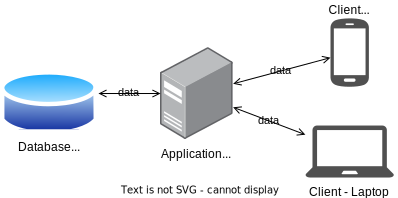
\includegraphics[width=\textwidth]{client-server-3-tier}
		\label{fig:client-server-schema}
		
		\column{0.4\textwidth}
		\begin{itemize}
			\item \textbf{Client Layer:} Provides the user interface.
			\item \textbf{Application Server:} Processes business logic.
			\item \textbf{Database Server:} Stores and retrieves data.
			\item \textbf{Benefits:} 
			\begin{itemize}
				\item Improved scalability
				\item Greater flexibility
				\item Better separation of concerns compared to the two-tier model
			\end{itemize}
		\end{itemize}
	\end{columns}
\end{frame}


\begin{frame}{Advantages of Client-Server Architecture}
	\begin{itemize}
		\item \textbf{Remote Accessibility:} Computing power and data storage can be accessed from multiple locations and by different users.
		\item \textbf{Delegation of Heavy Computation:} Tasks requiring high processing power can be offloaded to the server.
		\item \textbf{Centralized Data Management:} Ensures data consistency and reduces redundancy.
		\item \textbf{Scalability:}
		\begin{itemize}
			\item \textbf{Horizontal Scaling:} Adding more servers to distribute computational load.
			\item \textbf{Vertical Scaling:} Upgrading existing servers to improve performance.
		\end{itemize}
	\end{itemize}
\end{frame}

\begin{frame}{Challenges of Client-Server Architecture}
	\begin{itemize}
		\item \textbf{Higher Costs:} Additional hardware and infrastructure require more resources and maintenance.
		\item \textbf{Security Concerns:} Operating within a network increases exposure to cyber threats.
		\item \textbf{Coordination Between Components:} Requires careful synchronization of requests, parallel computations, and data consistency.
		\item \textbf{Compatibility Issues:} Ensuring smooth interaction between different client and server components can be complex.
		\item \textbf{Network-Related Issues:} Latency, misconfigurations, and connectivity failures can impact system performance.
	\end{itemize}
\end{frame}



	
	
	%	\begin{frame}{Defining Software Architecture}
		%	Software architecture consists of four components:
		%	\begin{itemize}
			%
			%		\item Structure (Architecture styles used)
			%		\begin{itemize}
				%			\item Structure refers to the type of architecture styles used in the system support.
				%		\end{itemize}
			%
			%		\item Architecture characteristics
			%		\begin{itemize}
				%			\item Architecture characteristics refers to the ``-ilities'' that the system must, e.g., availability, reliability, scalability, security, testability, etc.
				%		\end{itemize}
			%
			%
			%	\end{itemize}
		%\end{frame}
		%
		%	\begin{frame}{Defining Software Architecture (2)}
			%		Software architecture consists of four components:
			%		\begin{itemize}
				%
				%
				%			\item Architecture decisions
				%			\begin{itemize}
					%				\item Architecture decisions are rules for constructing systems. For example, database can only be accessed by the model layer in the MVC architecture.
					%			\end{itemize}
				%
				%			\item Design principles
				%			\begin{itemize}
					%				\item Design principles are guidelines for constructing systems, e.g, whenever possible, use asynchronous messaging.
					%			\end{itemize}
				%
				%		\end{itemize}
			%	\end{frame}
		%
		%	\begin{frame}{The Job Description of A Software Architect}
			%		\begin{itemize}
				%			\item Make architecture decisions
				%			\item Continually analyze the architecture
				%			\item Keep current with latest trends
				%			\item Ensure compliance with decisions
				%			\item Diverse exposure and experience
				%			\item Have business domain knowledge
				%			\item Possess interpersonal skills
				%			\item Understand and navigate politics
				%		\end{itemize}
			%	\end{frame}
		%
		%	\begin{frame}{Law of Software Architecture}
			%		\begin{itemize}
				%			\item Everything in software architecture is a trade-off.
				%			\item If architect thinks they have discovered something that is not a trade-off, more likely they just have not identified the trade-off yet.
				%			\item Why is more important than how.
				%		\end{itemize}
			%	\end{frame}
		%
		%	\begin{frame}{Architectural Characteristics}
			%		\begin{itemize}
				%			\item Operational Characteristics
				%			\begin{itemize}
					%				\item Availability, continuity (disaster recovery), performance, recoverability,
					%				reliability (1 - probability of failure), robustness, scalability
					%			\end{itemize}
				%			\item Structural Characteristics
				%			\begin{itemize}
					%				\item Configurability, extensibility, Installability, resusability, localization, maintainability, portability, supportability, Upgradeability
					%			\end{itemize}
				%
				%		\end{itemize}
			%	\end{frame}
		%
		%
		%	\begin{frame}{Architectural Characteristics(2)}
			%		\begin{itemize}
				%
				%			\item Cross-cutting Architecture Characteristics
				%			\begin{itemize}
					%				\item Accessibility, Archivability, authentication, authorization, legal, privacy, security,
					%				usability, supportability
					%			\end{itemize}
				%			\item ISO Characteristics
				%			\begin{itemize}
					%				\item performance efficiency, compatibility, usability, reliability, security, maintainability, portability, functional suitability (completeness, correctness, appropriateness)
					%			\end{itemize}
				%		\end{itemize}
			%	\end{frame}
		%
		%\begin{frame}{Background}
		%	\begin{itemize}
			%		\item Computer started as a single unit.  Software only ran on that single unit.
			%		\item The singular systems then gradually separated into different units, .i.e., for data storage and processing.
			%		\item Certain functionalities tend to grow overtime and require separate machines.
			%		\item Computer networking then became common. Different nodes can exchange messages with each other.
			%		\item Each node may have different roles.
			%		\item Distributed systems then appear.
			%	\end{itemize}
		%\end{frame}
		%
		%\begin{frame}{Client-Server}
		%	\begin{itemize}
			%		\item A client-server environment consists of, at least, a server and one or more clients.
			%		\item The server usually has more computing power than the clients.
			%		\item It receives request from the clients to perform certain tasks and then returns the results.
			%		\item Two-tier Architecture:
			%		\begin{itemize}
				%			\item Desktop apps + database server
				%			\item Browser + web server
				%		\end{itemize}
			%		\item Three-tier Architecture:
			%		\begin{itemize}
				%			\item Browser + application/web server + database server
				%		\end{itemize}
			%	\end{itemize}
		%\end{frame}
		%
		%\begin{frame}{Advantages}
		%	\begin{itemize}
			%		\item Computation can be accessed by multiple nodes/users from different remote locations.
			%		\item High-performance computation can be delegated to the server.
			%		\item Data can be centralised and therefore reduce data duplication.
			%		\item Scalable:
			%		\begin{itemize}
				%			\item Vertical scaling (upgrading a machine's specs)
				%			\item Horizontal scaling (adding more nodes/machines)
				%		\end{itemize}
			%	\end{itemize}
		%\end{frame}
		%
		%\begin{frame}{Disadvantages}
		%	\begin{itemize}
			%		\item More complex to manage:
			%		\begin{itemize}
				%			\item Cost (more components/machines to manage)
				%			\item Security (it operates in a network, prone to cyber attack)
				%			\item Coordination (e.g., async, sync, parallelism)
				%			\item Compatibility (e.g., different clients' specs)
				%			\item Network problems (e.g., latency)
				%		\end{itemize}
			%	\end{itemize}
		%\end{frame}
		%
		%\begin{frame}{Schema}
		%	\begin{figure}[h]
			%		\centering
			%		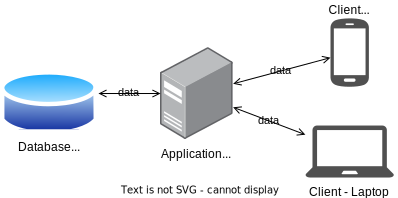
\includegraphics[width=0.6\textwidth]{client-server-3-tier}
			%		\caption{3-tier client-server architecture.}
			%		\label{fig:client-server-schema}
			%	\end{figure}
		%\end{frame}
		
	\end{document}
